 
We conducted a user study to examine the productivity of our system in constructing the digital 3D mockups from 2D layouts, and \xjmd{the effectiveness of our system of guiding non-expert users to fabricate the physical mockups from 2D layouts}. 
%
\xjmd{There are two experiments in our user study.}
% 
In the first experiment, participants were asked to construct the digital 3D model from the same 2D layout using our system and \xjmd{a commercial software} STUDIO, respectively, after a brief introduction.
\xjmd{For each participant, ten examples were randomly selected from the thirty-four 2D design layouts and presented to the participant for folding using our sytem and Studio.}
A \emph{two-alternative forced choices} design was used, with the participant asked to choose which of the two systems they prefer to use considering \xjmd{the operation simplicity and modeling efficiency}. 
%
Furthermore, participants were asked to rate our system from one to five on the necessity of layout optimization, while five \xjmd{indicates it is very necessary}. 


%
In the second experiment, participants were separated equally into two groups, one group was asked to fold \xjmd{a paper sheet with printed 2D layouts into a 3D mockup with the guide video showing the folding sequence provided by our system. Another group was asked to make a carton without the guide video. Each participant was assigned with the same 2D layout (Figure~\ref{fig:xxxx} (a)) because \cxj{provide the reason.}
%
The fabrication time was recorded for two groups.}
%
Our goal was to test the following hypotheses:

\begin{itemize}
	\item \textbf{Hypo1:} Our system need\xjmd{s} less time and effort to construct a digital 3D mockup than the traditional software.
	\item \textbf{Hypo2:} Our system \xjmd{provides more novel and practical functions to generate} diverse layouts.
	\item \textbf{Hypo3:} Our system \xjmd{is effective for guiding non-expert users to fabricate complex cartons from 2D layouts}.
\end{itemize}

\comments{
\subsection{Procedure}
We began the experiment with each participant by explaining the background and the instructions of our system and STUDIO. Ten layouts from thirty-four 2D design layouts were given to participants for folding, and at least three of them would need refinement. Participants were allowed to watch the final model of the layout to instruct construction. After operating the two systems. each participant was asked to answer a questionnaire including four(??five?? not clear how to use the question of modeling experiment) questions: which of two systems participants preferred based on the simplicity of operation. which of two systems participants preferred based on the modeling time, score one to five on the necessity of layout optimization in our system. and write down the suggestions to our system.

Foe the second experiment, we separated participants into two groups, one group would fabricate the layout as shown in Figure~\ref{fig:automatic-more}(a) with a video presenting the folding sequence, and another group would fold the layout with a figure showing the layout and its final model instead of video. The fabrication time was recorded for analysis.
}




%\subsection{Discussion}

We consider our three hypotheses in turn. 
With respect to \textbf{Hypo1}, we collect the answers of former two questions from 30 participants, \xjmd{all over eighteen years of age. 
	Both male and female participants were included, and none
	had any computer graphics background.??? }\cxj{Describe the background of participants. }
%
The result is shown in Figure~\ref{fig:preference}. 
\xjmd{The chart shows that $96\%$ of participants prefer our system considering the operation simplicity, and $96\%$ of participants prefer our system considering the modeling time.} \cxj{give the percentage number}
%
We also performed a paired-samples $t$-test at the level $\alpha = 0.05$ to compare the preference significance.
%
The test shows our system is significantly preferred by participants.
%
Most participants vote for our system mainly because it takes much less time to make a 3D model using our system. 
Take Figure~\ref{fig:result-more}(e) for example, participants usually spent much time on adjusting the folding angles of the creases, while only three clicks are required in our system.
%
On the other hand, one comment from the participants who prefer STUDIO is that the operation needed to be learned in STUDIO is just selecting a folding line and assigning angles, while our system requires them to learn more operations to construct the digital 3D model. 
%



\begin{figure}
	\centering
	\subfigure[Preference System]{
		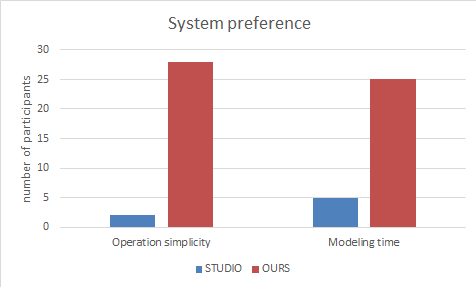
\includegraphics[width=0.45\columnwidth,height=0.17\textheight]{images/preference.png}
		\label{fig:preference}
	}
	\vspace{-1ex}
	\subfigure[Fabrication Time]{
		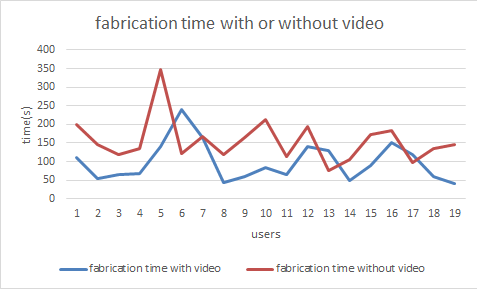
\includegraphics[width=0.45\columnwidth,height=0.17\textheight]{images/fabrication.png}
		\label{fig:time}
	}
	\caption{(a) shows the collection of the former two answers related to the preference based on modeling time and operation simplicity. (b) shows the fabrication time with or without video.  }
	\label{fig:data}
\end{figure}

With respect to \textbf{Hypo2}, twenty-four participants gave the highest score to our layout optimization function. 
%
In addition to explore the diversity of 2D layouts, it also can adjust the imprecise faces on the 2D layout to reach an ideal model by construction. Figure~\ref{fig:correction} shows the final model constructed by our system and STUDIO. As we can see, \cxj{Panel 1} is higher than $Panel_2$ in the digital model constructed by STUDIO, because of the 2D layout is not that precise. 
%
In comparison, our system is able to correct these design error by merging the 3D vertexes in different panels circled in red and optimizing the 2D layout simultaneously.

\begin{figure}
	\centering
	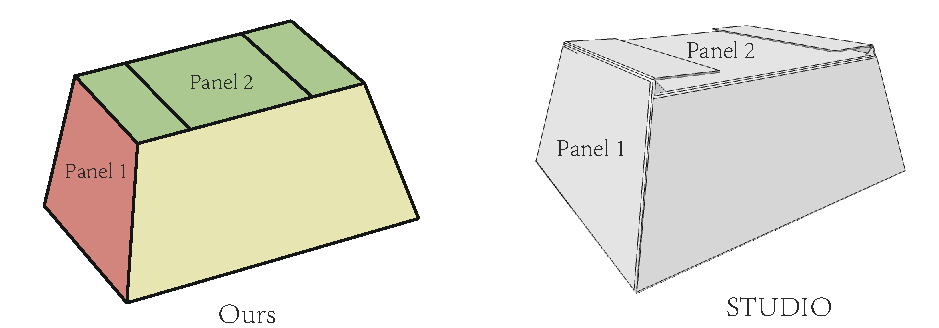
\includegraphics[width=0.5\textwidth]{images/comparison}
	\caption{Different model constructed by our system (a) and STUDIO (b). }
	\label{fig:correction}
\end{figure}

Considering \textbf{Hypo3}, 38 participants (19 for each group) were asked to fabricate the 2D layout shown in \cxj{Figxxx} into a physical mockup. 
The comparison of the fabrication times with and without our guide video is shown in Figure~\ref{fig:time}. 
As we can see, most participants who did not watch the guide video spent more time 
\cxj{averagely xxx seconds} to folding a carton than the other group \cxj{averagely xxx seconds }.
% 
%
We also performed an independent-samples t test at level $\alpha = 0.05$ to compare the fabrication time, and the result shows the guide video has significant effectiveness on the fabrication of complex cartons.




